\chapter{System Design}
This chapter portrays the design for the proposed implementation of the secure
ad hoc network.

\section{Requirements}
Ad hoc networks have some desired characteristics such as quick and inexpensive
setup and being independent of communication infrastructure, but they
also impose great challenges regarding security. The challenges
regarding security can vary depending the purpose and environment of the
network.

\subsection{Scenario}
The design and implementation presented in this thesis is mostly based on an
emergency situation scenario, in which communication infrastructure is
unavailable. This thesis will also reflect on some possible requirements given
by a military application.

If there is a major emergency situation such as an earthquake or tsunami, it is
likely that parts or the whole of the communication infrastructure at the scene
is destroyed or temporarily down. The remaining communication lines will then
probably be congested, such that little communication actually goes through.

In this situation, it is of great importance that Emergency Personnel, such as
Paramedics, Firemen, Policemen and the Military, are able to communicate
efficiently and therefore independently of the public communication
infrastructure. They need this network in order to manage the the operation, and
therefore availability is probably the most important trait of this network.
Secondly, they should be able to trust that the communication on the network is to be
trusted, i.e. messages sent are from whom they claim they to be.

Also, being able to authorize new actors on the scene, such as Red Cross, can be
critical to the operation. These new actors will probably not have the necessary
authentication tokens, i.e. certificates, required by the authentication scheme
in the network.

\subsection{List of Requirements}
Based on the scenario above these requirements can be extracted and made into
general requirements that needs to be addressed by the system design. The work
presented here is based on several sources, most prevalent being the research
from the OASIS project [OASIS] and the doctoral project of Eli Winjum carried
out at UniK \cite{ffi_2005_04015}.

\begin{table}[ht!]
	\centering
	\begin{tabular}{ | l | p{11cm} | }
	\hline
	\textbf{Requirement} & \textbf{Requirement Description}\\\hline
		R1 & A node must be authorized in order to get full rights in a
		network \cite{dahill2001secure}, \cite{sanzgiri2002secure}\\\hline
		R2 & A node without a recognized authentication token should be able to become
		authorized if necessary\\ \hline
		R3 & Networks need a master node which handles access control\\\hline
		R4 & Different networks should be able to collaborate
		\cite{ffi_2005_04015}\\\hline
	\end{tabular}
	\caption{Requirements based upon our simplified and general scenario.}
	\label{tab:our_req}
\end{table}

An early study produced security requirements of ad hoc networks demanding
that the routing logic must not be spoofed or altered to produce different
behavior \cite{dahill2001secure}. This means authorization is required (R1)
before someone can partake in routing logic. FFI also requires seamless radio coverage over the
area giving us R4.

\section{Design Overview}
The secure ad hoc network designed here does not change any fundamental workings
of regular ad hoc routing protocols. Assuming all nodes in the network already
have been authenticated, the routing in the network should behave as if there
were no secure extension to the routing protocol.

The proposed design should work with most pro-active ad hoc routing protocols
with limited alterations - but this design is specifically made for the
BATMAN \cite{batman_rfc} routing protocol chosen for its simpler design compared to
e.g. OLSR \cite{clausen2003rfc3626} because it only uses the third layer of the
OSI Model \cite{zimmermann1980osi}. How to incorporate this design into BATMAN will be
expained in Chapter \ref{chapter_implementation}.

The basic principle of the proposed design is that an authenticated node accepts
other authenticated nodes' routing messages and forwards them as normal, while
discarding routing messages from unauthenticated nodes. One or more nodes in the
network will assume a role as master node(s), with the extra capability of
authorizing new nodes into the network. A special certificate called a \ac{PC}
\cite{tuecke2004rfc3820} will be used for authentication after this authorization has taken
place so other nodes in the network will be able to authenticate and accept the new
node.


\subsection{Entity Explanation}

\begin{figure}[ht!]
	\centering
  	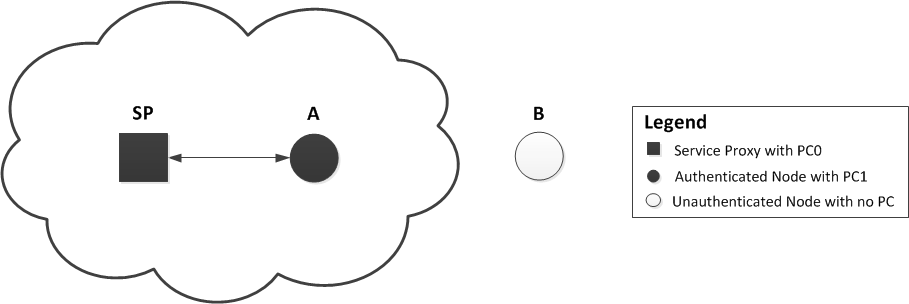
\includegraphics{images/simple_example_entities.png}
  	\caption{Different entities in the Simple Example.}
	\label{fig:simple_example_entities}
\end{figure}

Before a simplified example can be given, a few new entities to this design
needs to be explained further. This is the short version, just enough for the
reader to understand the example - the full description of these entities will
be given later.

\begin{itemize}
  \item \textbf{\acf{SP}} is responsible for tasks similar to that of a \ac{CA}
  	and has the master role in the network. The \ac{SP} is the entity that
 	 authorizes new nodes and signs their \acp{PC}.
  \item \textbf{\acf{PC0}} is a self-signed \ac{PC} belonging to a
  	\ac{SP}. This \ac{PC} has a certificate depth of 0, thus we refer to it as a
  	\ac{PC0}.
  \item \textbf{\acf{PC1}} is a \ac{PC} signed by a \ac{PC0} (i.e. the the
	 certificate of a \ac{SP}). All authenticated nodes in one network, has a
 	 \ac{PC1} signed by a \ac{SP} from that network.
  \item \textbf{\acf{AL}} is a list containing the necessary information about
 	all authorized nodes in the network. The \ac{SP} signs and broadcasts a copy
 	of the \ac{AL} periodically, and all nodes keep a local copy of the \ac{AL}
  	which they use to authenticate other nodes in the network.
  \item \textbf{Authenticated Node} bla bla.
  \item \textbf{Unauthenticated Node} bla bla.
\end{itemize}

\subsection{Simple Example}
Two nodes are within transmitting range of each other. One of the nodes is a
\ac{SP} and the other is unauthenticated. The pro-active ad hoc routing protocol
used on both nodes regularly broadcasts routing messages, so the two nodes learn
of each others' existence. Upon reception of a routing message from the
unauthenticated node, the \ac{SP} will invite the node for a handshake. With
this handshake, the unauthenticated node will send a self-generated \ac{PC}
which the \ac{SP} can sign as trusted - i.e. the node is issued a \ac{PC1}.

Before the \ac{SP} actually signs the \ac{PC} received from the unauthenticated
node, it needs some verification that the node is an actor that should be
allowed access to the network. The actor will therefore meet the \ac{SP} in the
field and give its \ac{PC}'s public key fingerprint (out-of-band) so the \ac{SP}
can verify the incoming \ac{PC} as the actor's.

Using the public key pair of the \ac{PC1}, the newly trusted node will now
broadcast a signature, and use an excerpt from this signature in its routing
messages. The \ac{SP}, recognizing the signature will rebroadcast the routing
messages so regular ad hoc routing follows.

Also upon handshake completion is the generation an \ac{AL}. The \ac{SP} will
use this list in order to save certain necessary details about the other node,
such as its address, public key, last signature, and more. Also in this list is
the corresponding information about the \ac{SP} itself. When the list is created
or updated it is broadcasted to the network - encrypted so its details stay
hidden from unauthenticated nodes.

Whenever a new node is discovered by the \ac{SP} this procedure repeats, and a
new addition is made to the \ac{AL}. Other previously trusted nodes will learn
the identity of new nodes when they receive the updated list from the \ac{SP}.

TODO: add an MSC or figure with the entities to explain the example\ldots

\section{Node States}
This section is devoted to explain the different states a node can be in, and
how it behaves during these different states. These states should be similar for
most pro-active routing protocols as the only thing triggering these phases are
the routing messages sent as per normal operation of any pro-active routing
protocol [some def of pro-active routing protocols\ldots].

\subsection{Node Discovery}
Upon entering the network area, the node is both unauthenticated and unknown to
the network.

\subsection{Authentication Handshake}

\subsection{Authorized Operation}